% Options for packages loaded elsewhere
\PassOptionsToPackage{unicode}{hyperref}
\PassOptionsToPackage{hyphens}{url}
%
\documentclass[
]{article}
\usepackage{amsmath,amssymb}
\usepackage{iftex}
\ifPDFTeX
  \usepackage[T1]{fontenc}
  \usepackage[utf8]{inputenc}
  \usepackage{textcomp} % provide euro and other symbols
\else % if luatex or xetex
  \usepackage{unicode-math} % this also loads fontspec
  \defaultfontfeatures{Scale=MatchLowercase}
  \defaultfontfeatures[\rmfamily]{Ligatures=TeX,Scale=1}
\fi
\usepackage{lmodern}
\ifPDFTeX\else
  % xetex/luatex font selection
\fi
% Use upquote if available, for straight quotes in verbatim environments
\IfFileExists{upquote.sty}{\usepackage{upquote}}{}
\IfFileExists{microtype.sty}{% use microtype if available
  \usepackage[]{microtype}
  \UseMicrotypeSet[protrusion]{basicmath} % disable protrusion for tt fonts
}{}
\makeatletter
\@ifundefined{KOMAClassName}{% if non-KOMA class
  \IfFileExists{parskip.sty}{%
    \usepackage{parskip}
  }{% else
    \setlength{\parindent}{0pt}
    \setlength{\parskip}{6pt plus 2pt minus 1pt}}
}{% if KOMA class
  \KOMAoptions{parskip=half}}
\makeatother
\usepackage{xcolor}
\usepackage[margin=1in]{geometry}
\usepackage{color}
\usepackage{fancyvrb}
\newcommand{\VerbBar}{|}
\newcommand{\VERB}{\Verb[commandchars=\\\{\}]}
\DefineVerbatimEnvironment{Highlighting}{Verbatim}{commandchars=\\\{\}}
% Add ',fontsize=\small' for more characters per line
\usepackage{framed}
\definecolor{shadecolor}{RGB}{248,248,248}
\newenvironment{Shaded}{\begin{snugshade}}{\end{snugshade}}
\newcommand{\AlertTok}[1]{\textcolor[rgb]{0.94,0.16,0.16}{#1}}
\newcommand{\AnnotationTok}[1]{\textcolor[rgb]{0.56,0.35,0.01}{\textbf{\textit{#1}}}}
\newcommand{\AttributeTok}[1]{\textcolor[rgb]{0.13,0.29,0.53}{#1}}
\newcommand{\BaseNTok}[1]{\textcolor[rgb]{0.00,0.00,0.81}{#1}}
\newcommand{\BuiltInTok}[1]{#1}
\newcommand{\CharTok}[1]{\textcolor[rgb]{0.31,0.60,0.02}{#1}}
\newcommand{\CommentTok}[1]{\textcolor[rgb]{0.56,0.35,0.01}{\textit{#1}}}
\newcommand{\CommentVarTok}[1]{\textcolor[rgb]{0.56,0.35,0.01}{\textbf{\textit{#1}}}}
\newcommand{\ConstantTok}[1]{\textcolor[rgb]{0.56,0.35,0.01}{#1}}
\newcommand{\ControlFlowTok}[1]{\textcolor[rgb]{0.13,0.29,0.53}{\textbf{#1}}}
\newcommand{\DataTypeTok}[1]{\textcolor[rgb]{0.13,0.29,0.53}{#1}}
\newcommand{\DecValTok}[1]{\textcolor[rgb]{0.00,0.00,0.81}{#1}}
\newcommand{\DocumentationTok}[1]{\textcolor[rgb]{0.56,0.35,0.01}{\textbf{\textit{#1}}}}
\newcommand{\ErrorTok}[1]{\textcolor[rgb]{0.64,0.00,0.00}{\textbf{#1}}}
\newcommand{\ExtensionTok}[1]{#1}
\newcommand{\FloatTok}[1]{\textcolor[rgb]{0.00,0.00,0.81}{#1}}
\newcommand{\FunctionTok}[1]{\textcolor[rgb]{0.13,0.29,0.53}{\textbf{#1}}}
\newcommand{\ImportTok}[1]{#1}
\newcommand{\InformationTok}[1]{\textcolor[rgb]{0.56,0.35,0.01}{\textbf{\textit{#1}}}}
\newcommand{\KeywordTok}[1]{\textcolor[rgb]{0.13,0.29,0.53}{\textbf{#1}}}
\newcommand{\NormalTok}[1]{#1}
\newcommand{\OperatorTok}[1]{\textcolor[rgb]{0.81,0.36,0.00}{\textbf{#1}}}
\newcommand{\OtherTok}[1]{\textcolor[rgb]{0.56,0.35,0.01}{#1}}
\newcommand{\PreprocessorTok}[1]{\textcolor[rgb]{0.56,0.35,0.01}{\textit{#1}}}
\newcommand{\RegionMarkerTok}[1]{#1}
\newcommand{\SpecialCharTok}[1]{\textcolor[rgb]{0.81,0.36,0.00}{\textbf{#1}}}
\newcommand{\SpecialStringTok}[1]{\textcolor[rgb]{0.31,0.60,0.02}{#1}}
\newcommand{\StringTok}[1]{\textcolor[rgb]{0.31,0.60,0.02}{#1}}
\newcommand{\VariableTok}[1]{\textcolor[rgb]{0.00,0.00,0.00}{#1}}
\newcommand{\VerbatimStringTok}[1]{\textcolor[rgb]{0.31,0.60,0.02}{#1}}
\newcommand{\WarningTok}[1]{\textcolor[rgb]{0.56,0.35,0.01}{\textbf{\textit{#1}}}}
\usepackage{graphicx}
\makeatletter
\def\maxwidth{\ifdim\Gin@nat@width>\linewidth\linewidth\else\Gin@nat@width\fi}
\def\maxheight{\ifdim\Gin@nat@height>\textheight\textheight\else\Gin@nat@height\fi}
\makeatother
% Scale images if necessary, so that they will not overflow the page
% margins by default, and it is still possible to overwrite the defaults
% using explicit options in \includegraphics[width, height, ...]{}
\setkeys{Gin}{width=\maxwidth,height=\maxheight,keepaspectratio}
% Set default figure placement to htbp
\makeatletter
\def\fps@figure{htbp}
\makeatother
\setlength{\emergencystretch}{3em} % prevent overfull lines
\providecommand{\tightlist}{%
  \setlength{\itemsep}{0pt}\setlength{\parskip}{0pt}}
\setcounter{secnumdepth}{-\maxdimen} % remove section numbering
\usepackage{booktabs}
\usepackage{caption}
\usepackage{longtable}
\usepackage{colortbl}
\usepackage{array}
\usepackage{anyfontsize}
\usepackage{multirow}
\ifLuaTeX
  \usepackage{selnolig}  % disable illegal ligatures
\fi
\usepackage{bookmark}
\IfFileExists{xurl.sty}{\usepackage{xurl}}{} % add URL line breaks if available
\urlstyle{same}
\hypersetup{
  pdftitle={Assignment 3: Collaborating in Github},
  pdfauthor={Brandon Yee; Veronica Leary},
  hidelinks,
  pdfcreator={LaTeX via pandoc}}

\title{Assignment 3: Collaborating in Github}
\author{Brandon Yee \and Veronica Leary}
\date{2025-03-24}

\begin{document}
\maketitle

\begin{center}\rule{0.5\linewidth}{0.5pt}\end{center}

\section{Introduction}\label{introduction}

This report generates and displays summary statistics of text message
counts by \textbf{Group} and \textbf{Time Point}.\\
We calculate measures of central tendency and variability to understand
texting patterns across two groups and over time.

\begin{center}\rule{0.5\linewidth}{0.5pt}\end{center}

\section{Load Required Libraries}\label{load-required-libraries}

\begin{Shaded}
\begin{Highlighting}[]
\FunctionTok{library}\NormalTok{(readr)          }\CommentTok{\# Reading CSV files}
\FunctionTok{library}\NormalTok{(gt)             }\CommentTok{\# Generating clean, styled summary tables}
\FunctionTok{library}\NormalTok{(ggplot2)        }\CommentTok{\# For plotting}
\FunctionTok{library}\NormalTok{(dplyr)          }\CommentTok{\# For data manipulation}
\FunctionTok{library}\NormalTok{(tidyr)          }\CommentTok{\# For reshaping data}
\FunctionTok{library}\NormalTok{(wesanderson)    }\CommentTok{\# For Wes Anderson{-}inspired color palettes}
\FunctionTok{library}\NormalTok{(reshape)        }\CommentTok{\# For converting data to long with melt()}
\end{Highlighting}
\end{Shaded}

\begin{center}\rule{0.5\linewidth}{0.5pt}\end{center}

\section{Data Loading and Cleaning}\label{data-loading-and-cleaning}

\begin{Shaded}
\begin{Highlighting}[]
\CommentTok{\# set working directory as folder on desktop}
 \FunctionTok{setwd}\NormalTok{(}\StringTok{"C:/Users/brand/OneDrive/Desktop/BHDS2010/ASSIGN3/bhds{-}assign{-}3"}\NormalTok{)}
\CommentTok{\# setwd("/Users/vleary71/Desktop/BHDS2010/ASSIGN3/bhds{-}assign{-}3")}
\CommentTok{\# successfully set working directory}

\CommentTok{\# Read in the dataset and clean header rows}
\NormalTok{data }\OtherTok{\textless{}{-}} \FunctionTok{read.csv}\NormalTok{(}\StringTok{"TextMessages.csv"}\NormalTok{)  }\CommentTok{\# Reads the dataset into an R dataframe}

\CommentTok{\# Reshape from wide to long format}
\NormalTok{data\_long }\OtherTok{\textless{}{-}}\NormalTok{ data }\SpecialCharTok{\%\textgreater{}\%}
  \FunctionTok{mutate}\NormalTok{(}\FunctionTok{across}\NormalTok{(}\FunctionTok{c}\NormalTok{(Baseline, Six\_months), as.numeric),}
         \AttributeTok{Group =} \FunctionTok{as.factor}\NormalTok{(Group)) }\SpecialCharTok{\%\textgreater{}\%}
  \FunctionTok{pivot\_longer}\NormalTok{(}\AttributeTok{cols =} \FunctionTok{c}\NormalTok{(Baseline, Six\_months),}
               \AttributeTok{names\_to =} \StringTok{"Time"}\NormalTok{,}
               \AttributeTok{values\_to =} \StringTok{"TextMessages"}\NormalTok{)}
\end{Highlighting}
\end{Shaded}

\begin{center}\rule{0.5\linewidth}{0.5pt}\end{center}

\section{Summary Statistics
Calculation}\label{summary-statistics-calculation}

We calculate:

\begin{itemize}
\tightlist
\item
  \textbf{Count} of observations per group/time
\item
  \textbf{Mean}, \textbf{Median}, and \textbf{Standard Deviation} of
  text message counts
\end{itemize}

\begin{Shaded}
\begin{Highlighting}[]
\NormalTok{summary\_table }\OtherTok{\textless{}{-}}\NormalTok{ data\_long }\SpecialCharTok{\%\textgreater{}\%}
  \FunctionTok{group\_by}\NormalTok{(Group, Time) }\SpecialCharTok{\%\textgreater{}\%}
  \FunctionTok{summarise}\NormalTok{(}
    \AttributeTok{Count =} \FunctionTok{n}\NormalTok{(),}
    \AttributeTok{Mean =} \FunctionTok{round}\NormalTok{(}\FunctionTok{mean}\NormalTok{(TextMessages, }\AttributeTok{na.rm =} \ConstantTok{TRUE}\NormalTok{), }\DecValTok{2}\NormalTok{),}
    \AttributeTok{Median =} \FunctionTok{round}\NormalTok{(}\FunctionTok{median}\NormalTok{(TextMessages, }\AttributeTok{na.rm =} \ConstantTok{TRUE}\NormalTok{), }\DecValTok{2}\NormalTok{),}
    \AttributeTok{SD =} \FunctionTok{round}\NormalTok{(}\FunctionTok{sd}\NormalTok{(TextMessages, }\AttributeTok{na.rm =} \ConstantTok{TRUE}\NormalTok{), }\DecValTok{2}\NormalTok{),}
    \AttributeTok{.groups =} \StringTok{"drop"}
\NormalTok{  )}
\end{Highlighting}
\end{Shaded}

\begin{center}\rule{0.5\linewidth}{0.5pt}\end{center}

\section{Summary Table Output}\label{summary-table-output}

\begin{Shaded}
\begin{Highlighting}[]
\NormalTok{summary\_table }\SpecialCharTok{\%\textgreater{}\%}
  \FunctionTok{gt}\NormalTok{() }\SpecialCharTok{\%\textgreater{}\%}
  \FunctionTok{tab\_header}\NormalTok{(}
    \AttributeTok{title =} \StringTok{"Summary Statistics of Text Messages"}\NormalTok{,}
    \AttributeTok{subtitle =} \StringTok{"Grouped by Treatment Group and Time Point"}
\NormalTok{  ) }\SpecialCharTok{\%\textgreater{}\%}
  \FunctionTok{cols\_label}\NormalTok{(}
    \AttributeTok{Group =} \StringTok{"Group"}\NormalTok{,}
    \AttributeTok{Time =} \StringTok{"Time Point"}\NormalTok{,}
    \AttributeTok{Count =} \StringTok{"N"}\NormalTok{,}
    \AttributeTok{Mean =} \StringTok{"Mean"}\NormalTok{,}
    \AttributeTok{Median =} \StringTok{"Median"}\NormalTok{,}
    \AttributeTok{SD =} \StringTok{"Standard Deviation"}
\NormalTok{  ) }\SpecialCharTok{\%\textgreater{}\%}
  \FunctionTok{fmt\_number}\NormalTok{(}\AttributeTok{columns =} \FunctionTok{c}\NormalTok{(Mean, Median, SD), }\AttributeTok{decimals =} \DecValTok{2}\NormalTok{) }\SpecialCharTok{\%\textgreater{}\%}
  \FunctionTok{tab\_options}\NormalTok{(}
    \AttributeTok{table.font.size =} \DecValTok{12}\NormalTok{,}
    \AttributeTok{heading.title.font.size =} \DecValTok{16}\NormalTok{,}
    \AttributeTok{heading.subtitle.font.size =} \DecValTok{14}
\NormalTok{  )}
\end{Highlighting}
\end{Shaded}

\begin{table}[!t]
\caption*{
{\large Summary Statistics of Text Messages} \\ 
{\small Grouped by Treatment Group and Time Point}
} 
\fontsize{9.0pt}{10.8pt}\selectfont
\begin{tabular*}{\linewidth}{@{\extracolsep{\fill}}clrrrr}
\toprule
Group & Time Point & N & Mean & Median & Standard Deviation \\ 
\midrule\addlinespace[2.5pt]
1 & Baseline & 25 & 64.84 & 64.00 & 10.68 \\ 
1 & Six\_months & 25 & 52.96 & 58.00 & 16.33 \\ 
2 & Baseline & 25 & 65.60 & 65.00 & 10.84 \\ 
2 & Six\_months & 25 & 61.84 & 62.00 & 9.41 \\ 
\bottomrule
\end{tabular*}
\end{table}

\begin{center}\rule{0.5\linewidth}{0.5pt}\end{center}

\section{Inference}\label{inference}

\begin{itemize}
\tightlist
\item
  If the \textbf{mean} and \textbf{median} differ substantially, this
  may suggest skewness in message volume.
\item
  Compare between \textbf{Groups} to explore differences in texting
  behavior.
\item
  An increase from \textbf{Baseline} to \textbf{Six\_months} may
  indicate behavioral changes over time.
\item
  Use standard deviation to understand variability within each subgroup.
\end{itemize}

\begin{Shaded}
\begin{Highlighting}[]
\DocumentationTok{\#\#\#Visualization 1:}
\CommentTok{\#Stratified boxplot of text messages by Group and Time}
\CommentTok{\#Hint: Faceted Boxplot}

\CommentTok{\#Read data set in}
\CommentTok{\#Use read.csv since the file is a csv file}
\NormalTok{text\_data }\OtherTok{\textless{}{-}} \FunctionTok{read.csv}\NormalTok{(}\StringTok{"TextMessages.csv"}\NormalTok{)}
\CommentTok{\#File was successfully read in}

\CommentTok{\#Use nrow() to check the number of rows/observations}
\FunctionTok{nrow}\NormalTok{(text\_data)}
\end{Highlighting}
\end{Shaded}

\begin{verbatim}
## [1] 50
\end{verbatim}

\begin{Shaded}
\begin{Highlighting}[]
\CommentTok{\#There are 50 rows in the dataset}

\CommentTok{\#Use names() to view the variable names}
\FunctionTok{names}\NormalTok{(text\_data)}
\end{Highlighting}
\end{Shaded}

\begin{verbatim}
## [1] "Group"       "Baseline"    "Six_months"  "Participant"
\end{verbatim}

\begin{Shaded}
\begin{Highlighting}[]
\CommentTok{\#There are variables "Group", "Baseline", "Six\_months" and "Participant"}

\CommentTok{\#Using cbind to combine the melted text data without the Group variable with a}
\CommentTok{\#a column containing the Group variable replicated a second time.}
\NormalTok{long\_text\_data }\OtherTok{\textless{}{-}} \FunctionTok{cbind}\NormalTok{(}\FunctionTok{melt}\NormalTok{(text\_data[,}\SpecialCharTok{{-}}\DecValTok{1}\NormalTok{],}
                             \AttributeTok{id.vars =} \StringTok{"Participant"}\NormalTok{, }\CommentTok{\#not melting Participant}
                             \AttributeTok{variable\_name =} \StringTok{"Time"}\NormalTok{, }\CommentTok{\#Variable name for melted}
                       \AttributeTok{value.names =} \StringTok{"Texts"}\NormalTok{), }\CommentTok{\#argument not working? Supposed}
                       \CommentTok{\#to change the variable name to "Texts", but doesn\textquotesingle{}t }
                       \CommentTok{\#seem to work anymore.}
                       \AttributeTok{Group =} \FunctionTok{rep}\NormalTok{(text\_data}\SpecialCharTok{$}\NormalTok{Group, }\DecValTok{2}\NormalTok{)) }\CommentTok{\#Using rep() to replicate}

\CommentTok{\#Use is.factor() to check if Group is a factor}
\FunctionTok{is.factor}\NormalTok{(long\_text\_data}\SpecialCharTok{$}\NormalTok{Group)}
\end{Highlighting}
\end{Shaded}

\begin{verbatim}
## [1] FALSE
\end{verbatim}

\begin{Shaded}
\begin{Highlighting}[]
\CommentTok{\#FALSE was returned}
\CommentTok{\#Use as.factor() to change it to a factor}
\NormalTok{long\_text\_data}\SpecialCharTok{$}\NormalTok{Group }\OtherTok{\textless{}{-}} \FunctionTok{as.factor}\NormalTok{(long\_text\_data}\SpecialCharTok{$}\NormalTok{Group)}
\CommentTok{\#Verify again with is.factor()}
\FunctionTok{is.factor}\NormalTok{(long\_text\_data}\SpecialCharTok{$}\NormalTok{Group)}
\end{Highlighting}
\end{Shaded}

\begin{verbatim}
## [1] TRUE
\end{verbatim}

\begin{Shaded}
\begin{Highlighting}[]
\CommentTok{\#TRUE is returned this time}

\CommentTok{\#Check if Time is a factor with is.factor()}
\FunctionTok{is.factor}\NormalTok{(long\_text\_data}\SpecialCharTok{$}\NormalTok{Time)}
\end{Highlighting}
\end{Shaded}

\begin{verbatim}
## [1] TRUE
\end{verbatim}

\begin{Shaded}
\begin{Highlighting}[]
\CommentTok{\#TRUE was returned}

\CommentTok{\#Check the factor names of Time using levels()}
\FunctionTok{levels}\NormalTok{(long\_text\_data}\SpecialCharTok{$}\NormalTok{Time)}
\end{Highlighting}
\end{Shaded}

\begin{verbatim}
## [1] "Baseline"   "Six_months"
\end{verbatim}

\begin{Shaded}
\begin{Highlighting}[]
\CommentTok{\#"Baseline" and "Six\_months" were returned}

\CommentTok{\#Use levels again and set the names of the factors to have "Six Months" for}
\CommentTok{\#easier readability for the boxplots}
\FunctionTok{levels}\NormalTok{(long\_text\_data}\SpecialCharTok{$}\NormalTok{Time) }\OtherTok{\textless{}{-}} \FunctionTok{c}\NormalTok{(}\StringTok{"Baseline"}\NormalTok{, }\StringTok{"Six Months"}\NormalTok{)}
\CommentTok{\#check the levels again}
\FunctionTok{levels}\NormalTok{(long\_text\_data}\SpecialCharTok{$}\NormalTok{Time)}
\end{Highlighting}
\end{Shaded}

\begin{verbatim}
## [1] "Baseline"   "Six Months"
\end{verbatim}

\begin{Shaded}
\begin{Highlighting}[]
\CommentTok{\#Now "Baseline" and "Six Months" was returned}


\DocumentationTok{\#\#\#\#\#\#Plot the boxplots}

\CommentTok{\#Use ggplot() with aes set for group on x to stratify and value on y with}
\CommentTok{\#fill = group to allow the plots to be colored}
\FunctionTok{ggplot}\NormalTok{(long\_text\_data, }\FunctionTok{aes}\NormalTok{(}\AttributeTok{x=}\NormalTok{Group, }\AttributeTok{y =}\NormalTok{ value, }\AttributeTok{fill =}\NormalTok{ Group)) }\SpecialCharTok{+} 
  \CommentTok{\#adding a boxplot with geom\_boxplot()}
  \FunctionTok{geom\_boxplot}\NormalTok{() }\SpecialCharTok{+}
  \CommentTok{\#Use facet\_wrap() to stratify the boxplots by time}
  \FunctionTok{facet\_wrap}\NormalTok{(.}\SpecialCharTok{\textasciitilde{}}\NormalTok{Time) }\SpecialCharTok{+}
  \CommentTok{\#add labels for the title and y axis}
  \FunctionTok{labs}\NormalTok{(}\AttributeTok{title =} \StringTok{"Boxplots of Text Data Stratified by Group and Time"}\NormalTok{,}
       \AttributeTok{y =} \StringTok{"Total Text Messages"}\NormalTok{)}\SpecialCharTok{+} 
  \CommentTok{\#adding a color to the boxplots}
  \FunctionTok{scale\_fill\_brewer}\NormalTok{(}\AttributeTok{palette =} \StringTok{"Pastel1"}\NormalTok{) }\SpecialCharTok{+} 
  \CommentTok{\#centering the title of the plot}
  \FunctionTok{theme}\NormalTok{(}\AttributeTok{plot.title =} \FunctionTok{element\_text}\NormalTok{(}\AttributeTok{hjust =} \FloatTok{0.5}\NormalTok{))}
\end{Highlighting}
\end{Shaded}

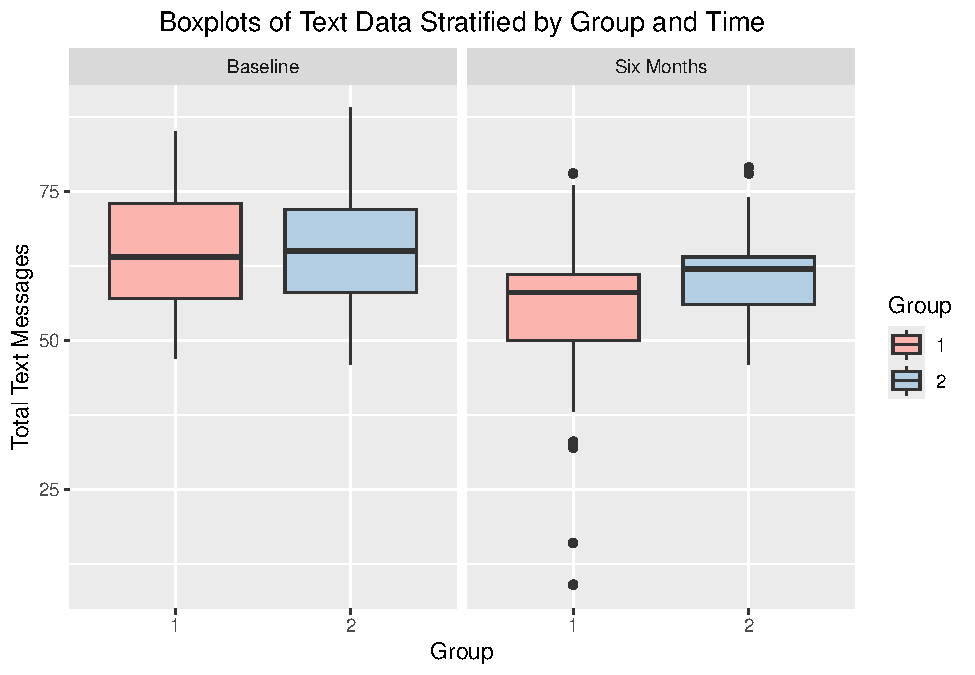
\includegraphics{Assignment_3_Collaborating_in_Github_files/figure-latex/Visual 1 Stratified Boxplot-1.pdf}

\begin{Shaded}
\begin{Highlighting}[]
\CommentTok{\#The figure was successfully created}
\end{Highlighting}
\end{Shaded}

\begin{Shaded}
\begin{Highlighting}[]
\DocumentationTok{\#\#\#Visualization 2:}
\CommentTok{\# stratified\_bar\_chart.R}
\CommentTok{\# Stratified Bar Chart of Text Messages by Group and Time}
\CommentTok{\# Author: Collaborative GitHub Project Team/Veronica Leary}
\CommentTok{\# Description: This script generates a stratified bar chart with a Wes Anderson }
\CommentTok{\#color palette using ggplot2 and dplyr}

\CommentTok{\# Load and clean the dataset}
\NormalTok{data }\OtherTok{\textless{}{-}} \FunctionTok{read.csv}\NormalTok{(}\StringTok{"TextMessages.csv"}\NormalTok{)  }\CommentTok{\# Load dataset}

\CommentTok{\# Rename columns for clarity}
\FunctionTok{colnames}\NormalTok{(data) }\OtherTok{\textless{}{-}} \FunctionTok{c}\NormalTok{(}\StringTok{"Group"}\NormalTok{, }\StringTok{"Baseline"}\NormalTok{, }\StringTok{"Six\_months"}\NormalTok{, }\StringTok{"Participant"}\NormalTok{)}

\CommentTok{\# Remove redundant header row}
\NormalTok{data }\OtherTok{\textless{}{-}}\NormalTok{ data[}\SpecialCharTok{{-}}\DecValTok{1}\NormalTok{, ]}

\CommentTok{\# Convert data types and reshape}
\NormalTok{data }\OtherTok{\textless{}{-}}\NormalTok{ data }\SpecialCharTok{\%\textgreater{}\%}
  \FunctionTok{mutate}\NormalTok{(}\FunctionTok{across}\NormalTok{(}\FunctionTok{c}\NormalTok{(Baseline, Six\_months), as.numeric),}
         \AttributeTok{Group =} \FunctionTok{as.factor}\NormalTok{(Group)) }\SpecialCharTok{\%\textgreater{}\%}
  \FunctionTok{pivot\_longer}\NormalTok{(}\AttributeTok{cols =} \FunctionTok{c}\NormalTok{(Baseline, Six\_months),}
               \AttributeTok{names\_to =} \StringTok{"Time"}\NormalTok{,}
               \AttributeTok{values\_to =} \StringTok{"TextMessages"}\NormalTok{)}
\end{Highlighting}
\end{Shaded}

\begin{Shaded}
\begin{Highlighting}[]
\CommentTok{\#Use ggplot() with pipeline and dplyr set as groups 1 and 2 and stratified by }
\CommentTok{\#two points in time{-}at basline and six months (x{-}axis) and assessed by the }
\CommentTok{\#number of text messages (y{-}axis) with text messages ranging from 0 to 1500}
\NormalTok{data }\SpecialCharTok{\%\textgreater{}\%}
  \FunctionTok{group\_by}\NormalTok{(Group, Time) }\SpecialCharTok{\%\textgreater{}\%}
  \FunctionTok{summarise}\NormalTok{(}\AttributeTok{TotalMessages =} \FunctionTok{sum}\NormalTok{(TextMessages, }\AttributeTok{na.rm =} \ConstantTok{TRUE}\NormalTok{), }\AttributeTok{.groups =} \StringTok{"drop"}\NormalTok{) }\SpecialCharTok{\%\textgreater{}\%}
  \FunctionTok{ggplot}\NormalTok{(}\FunctionTok{aes}\NormalTok{(}\AttributeTok{x =}\NormalTok{ Time, }\AttributeTok{y =}\NormalTok{ TotalMessages, }\AttributeTok{fill =}\NormalTok{ Group)) }\SpecialCharTok{+}
  \FunctionTok{geom\_bar}\NormalTok{(}\AttributeTok{stat =} \StringTok{"identity"}\NormalTok{, }\AttributeTok{position =} \StringTok{"dodge"}\NormalTok{) }\SpecialCharTok{+}
  \FunctionTok{facet\_wrap}\NormalTok{(}\SpecialCharTok{\textasciitilde{}}\NormalTok{ Group) }\SpecialCharTok{+}
  \FunctionTok{scale\_fill\_manual}\NormalTok{(}\AttributeTok{values =} \FunctionTok{wes\_palette}\NormalTok{(}\StringTok{"Rushmore"}\NormalTok{, }\AttributeTok{n =} \DecValTok{2}\NormalTok{)) }\SpecialCharTok{+}
  \FunctionTok{labs}\NormalTok{(}\AttributeTok{title =} \StringTok{"Stratified Bar Chart of Text Messages by Group and Time"}\NormalTok{,}
       \AttributeTok{x =} \StringTok{"Time Point"}\NormalTok{,}
       \AttributeTok{y =} \StringTok{"Total Text Messages"}\NormalTok{) }\SpecialCharTok{+}
  \FunctionTok{theme\_minimal}\NormalTok{(}\AttributeTok{base\_size =} \DecValTok{14}\NormalTok{) }\SpecialCharTok{+}
  \FunctionTok{theme}\NormalTok{(}\AttributeTok{legend.position =} \StringTok{"none"}\NormalTok{)}
\end{Highlighting}
\end{Shaded}

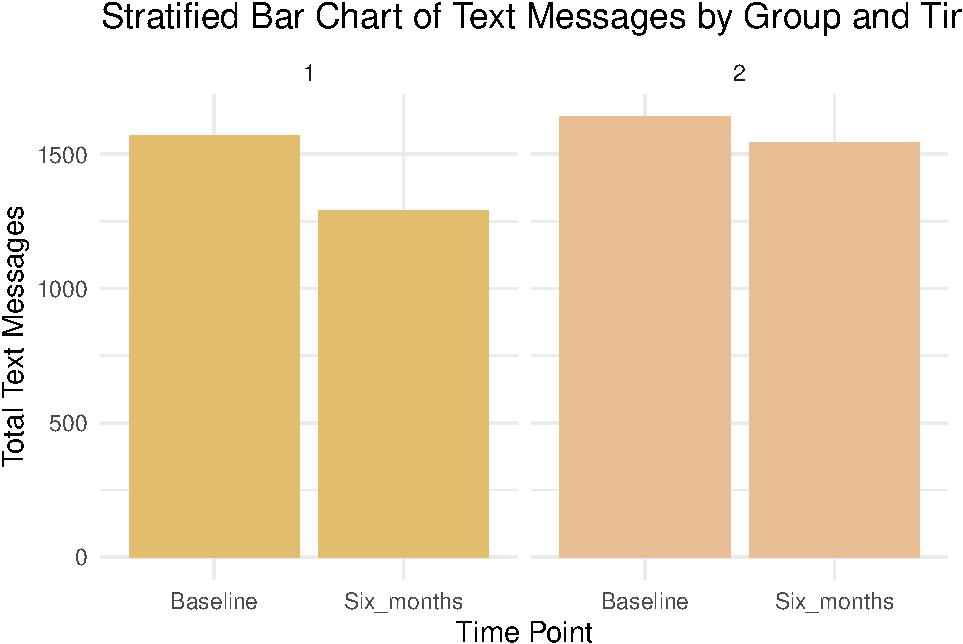
\includegraphics{Assignment_3_Collaborating_in_Github_files/figure-latex/Bar Chart-1.pdf}

\section{Project Summary}\label{project-summary}

\section{This script outlines the contributions and workflow from our
group project analyzing text message
data.}\label{this-script-outlines-the-contributions-and-workflow-from-our-group-project-analyzing-text-message-data.}

\section{It can be used as a reference in combination with the visual
and statistical output
scripts.}\label{it-can-be-used-as-a-reference-in-combination-with-the-visual-and-statistical-output-scripts.}

\section{Contributions Overview}\label{contributions-overview}

\section{Brandon Yee:}\label{brandon-yee}

\#- Responsible for initial setup of Github repository \#- Responsible
for Visualization 1: Stratified boxplot using ggplot2 default theme. \#
- This visualization highlighted the distribution of text messages
across time and group, \# including medians, variability, and outliers.
\#- Responsible originally for summary statistics: \# - Wrote code for
summary statistics using stat.desc and by functions. \# - Deferred and
handed off to Veronica since she had a more aesthetic display method.

\section{Veronica Leary:}\label{veronica-leary}

\section{- Responsible for Visualization 2: Stratified bar chart using
ggplot2 + wesanderson
theme.}\label{responsible-for-visualization-2-stratified-bar-chart-using-ggplot2-wesanderson-theme.}

\section{- Allowed for comparison of total message counts between groups
and time
points.}\label{allowed-for-comparison-of-total-message-counts-between-groups-and-time-points.}

\section{- Revealed possible increase in message volume in Group B over
time.}\label{revealed-possible-increase-in-message-volume-in-group-b-over-time.}

\section{- Responsible for Summary
Statistics:}\label{responsible-for-summary-statistics}

\section{- Used dplyr + gt to produce a well-formatted table of N, Mean,
Median, and
SD.}\label{used-dplyr-gt-to-produce-a-well-formatted-table-of-n-mean-median-and-sd.}

\section{- Supported the interpretation of patterns observed in the
plots.}\label{supported-the-interpretation-of-patterns-observed-in-the-plots.}

\section{- Responsible for all
documentation:}\label{responsible-for-all-documentation}

\section{- Embedded interpretation and narrative into
visualizations.}\label{embedded-interpretation-and-narrative-into-visualizations.}

\section{- Created markdown and final report files for
submission.}\label{created-markdown-and-final-report-files-for-submission.}

\begin{Shaded}
\begin{Highlighting}[]
\CommentTok{\# GitHub Workflow}
\end{Highlighting}
\end{Shaded}

\section{GitHub Workflow}\label{github-workflow}

\section{- Created a dedicated branch for visualizations and
documentation
tasks.}\label{created-a-dedicated-branch-for-visualizations-and-documentation-tasks.}

\section{- Commit messages included:}\label{commit-messages-included}

\section{- ``Added stratified bar chart with Wes Anderson color
palette''}\label{added-stratified-bar-chart-with-wes-anderson-color-palette}

\section{- ``Generated summary statistics table with
gt''}\label{generated-summary-statistics-table-with-gt}

\section{- ``Created documentation and embedded inference
blocks''}\label{created-documentation-and-embedded-inference-blocks}

\section{- Pushes were successful, but merge is pending due to
repository
permissions}\label{pushes-were-successful-but-merge-is-pending-due-to-repository-permissions}

\section{(partner is the owner of the GitHub
repo).}\label{partner-is-the-owner-of-the-github-repo.}

\section{- Push to main branch by Brandon was successful after he
reviewed and
edited.}\label{push-to-main-branch-by-brandon-was-successful-after-he-reviewed-and-edited.}

\section{Reflection}\label{reflection}

\section{This assignment helped
reinforce:}\label{this-assignment-helped-reinforce}

\section{- The value of clear commit messages and reproducible
code.}\label{the-value-of-clear-commit-messages-and-reproducible-code.}

\section{- Collaborative coding practices using Git and
GitHub.}\label{collaborative-coding-practices-using-git-and-github.}

\section{- Communicating visual and statistical insights clearly through
embedded
narrative.}\label{communicating-visual-and-statistical-insights-clearly-through-embedded-narrative.}

\end{document}
